\section{Latent Diffusion and Stable Diffusion}

\begin{frame}[plain]
    \centering
    \vspace{2cm}
    {\Huge \textcolor{blue}{Stable Diffusion:}\\[1em]
     \textbf{A Latent Diffusion Model (LDM)}}
\end{frame}

\begin{frame}{Perceptual vs.\ Semantic Compression}
  Pixel-space diffusion is redundant: the U-Net spends capacity on imperceptible high-frequency detail.
  \textbf{Stable Diffusion} (Rombach et al., 2022) decouples:
  \begin{enumerate}
    \item \textbf{Perceptual compression (VAE):} $\mathcal{E}: \mathbf{x} \mapsto \mathbf{z}$; remove imperceptible spatial detail, preserve layout.
    \item \textbf{Semantic generation (LDM):} run diffusion on $\mathbf{z}$; lower memory, faster training.
    \item \textbf{Decode:} $\mathcal{D}(\mathbf{z}) \mapsto \mathbf{x}$; project back to pixels.
  \end{enumerate}
  Typical spatial downsampling: $8\times$ (e.g., $512 \times 512 \times 3$ pixels $\rightarrow$ $64 \times 64 \times 4$ latents, a $\sim$48$\times$ reduction in dimensions).
\end{frame}

\begin{frame}{Cross-Attention: Injecting Text into the U-Net}
  \textbf{Pipeline:} CLIP text encoder $\rightarrow$ token embeddings $\mathbf{c} \in \mathbb{R}^{L \times d}$.
  \begin{itemize}
    \item \textbf{Self-attention:} Q, K, V all come from spatial latent features; provides global visual coherence.
    \item \textbf{Cross-attention:} Q from spatial features; K, V from the text embeddings; aligns latent spatial positions with prompt tokens.
  \end{itemize}
  \[
    \mathrm{Attention}(Q, K, V) = \mathrm{softmax}\!\left(\frac{QK^\top}{\sqrt{d_k}}\right) V
  \]
  Scaling by $\sqrt{d_k}$ prevents softmax saturation in high dimensions.\\[0.3em]
  {\footnotesize Token length $L \leq 77$ (CLIP); multi-head attention throughout the U-Net blocks.}
\end{frame}

\begin{frame}[allowframebreaks]{What is a Latent Space?}
    \begin{figure}
        \centering
        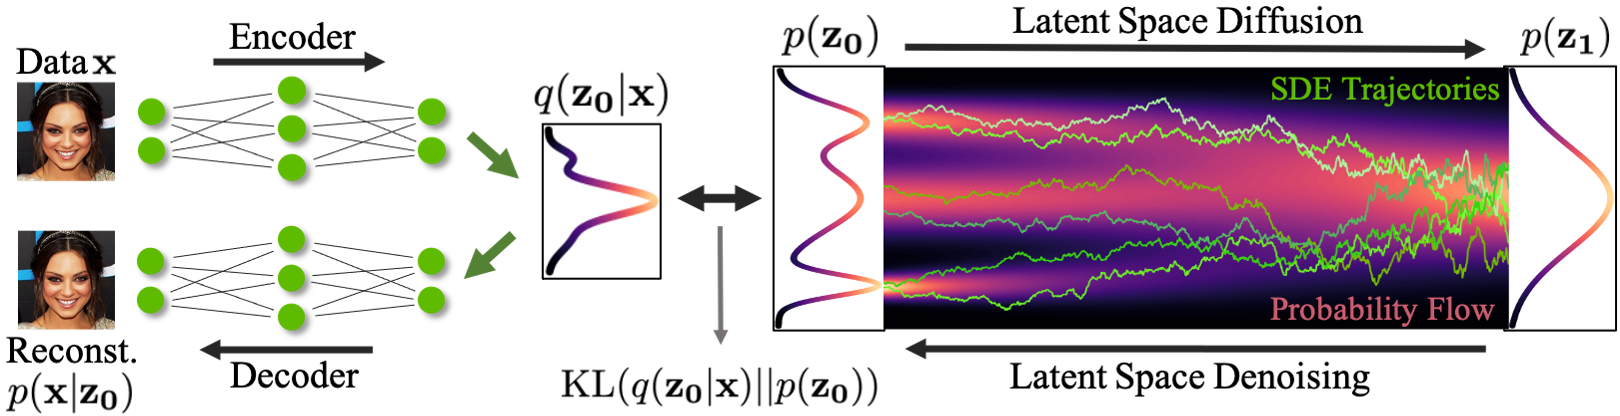
\includegraphics[width=\textwidth,height=0.25\textheight,keepaspectratio]{images/diffusion/latent-space-diffusion.png}
        \caption*{\scriptsize Vahdat, Kreis \& Kautz, \href{https://arxiv.org/abs/2106.05931}{Score-based Generative Modeling in Latent Space}, NeurIPS 2021, Fig.~1}
    \end{figure}
    \begin{itemize}
        \setlength{\itemsep}{-0.5em}
        \item A \textbf{latent space} is an abstract, compressed space where high-dimensional data (like images) is represented in a lower-dimensional form.
        \item Think of it as a hidden layer of meaning: each point in this space represents a potential image or concept.
        \item In classical models like GANs or VAEs, the latent space is directly sampled from (e.g., a vector $\mathbf{z}$), and the generator turns it into an image.
        \item \textbf{Latent} space = ``Hidden space of ideas or features''
        \item Note that even a pixel-space diffusion model has a latent code: the initial noise vector. Changing it gives a different image, and interpolating it morphs between images.
    \end{itemize}
\end{frame}

\begin{frame}{Why Latent Diffusion?}
    \begin{itemize}
        \item \textbf{Traditional pixel-space diffusion models are computationally expensive}: they operate directly on high-dimensional images, making both training and inference costly.
        \item \textbf{Latent diffusion reduces computational cost} by performing the diffusion process in a compressed, lower-dimensional latent space, while still maintaining high-quality image generation.
        \item This efficiency enables more complex and practical applications, such as text-guided generation and flexible image editing.
        \item \textbf{How is this achieved?} Instead of working in pixel space, we learn a compressed latent space using a Variational Autoencoder (VAE) with very low KL divergence weight (e.g., $10^{-6}$). This yields a compact representation suitable for diffusion.
        \item This mirrors the two-stage recipe of VQGAN: compress to a discrete or continuous code with an autoencoder, then model the distribution over that code.
    \end{itemize}
\end{frame}

\begin{frame}{Latent Diffusion Models: Visual Overview}
    \begin{figure}
        \centering
        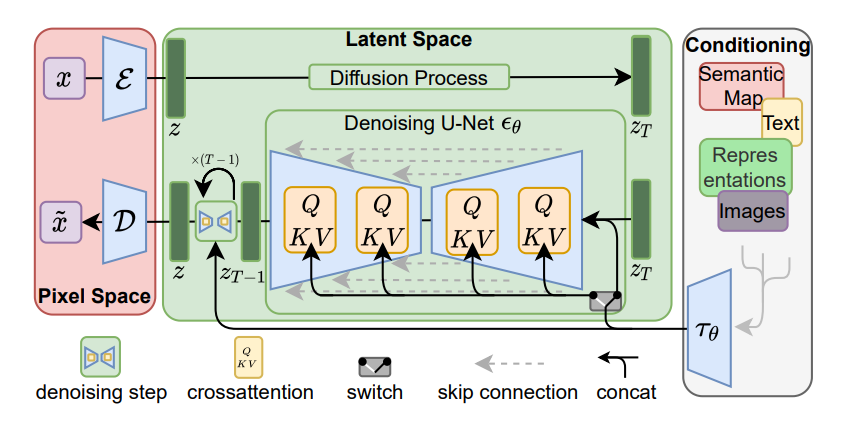
\includegraphics[width=\linewidth,height=0.78\textheight,keepaspectratio]{images/adv-img-gen/ldm_architecture_rombach.png}
        \caption*{\scriptsize Source: Rombach et al., ``High-Resolution Image Synthesis with Latent Diffusion Models'', CVPR 2022, Fig.~3.}
    \end{figure}
\end{frame}

